
\chapter{Implementacja}

\section{REST API}
REST API jest to interfejs służący do komunikacji między Backendem i Frontendem, przez to realizując architekturę klient-serwer. W naszym projekcie został zaimplementowany 
za pomocą frameworka Spring Boot. Dzięki niemu możliwa była wydajna i prosta integracja z bazą danych PostgreSQL, która jest istotnym
punktem naszego systemu. Użycie Spring Boota umożliwiło zastosowanie operacji CRUD, które z kolei są możliwe do implementacji dzięki 
metodom HTTP takim jak: GET, PUT, POST, DELETE. Ważna cecha jaką jest warstwowość pozwoliła nam na oddzielenie części aplikacji:
\begin{itemize}
    \item warstwa prezencji - składa się z kontrolerów, z których zarówno może korzystać frontend oraz inne serwisy.
    \item warstwa serwisowa - składająca się z serwisów, które odpowiadają za logikę biznesową aplikacji
    \item warstwa dostępu do danych - składają się z repozytoriów, które odpowiadają za operacje na bazie danych
    \item warstwa infastrukturalna - składająca się z wielu komponentów, odpowiedzialnych głównie za konfigurację oraz kontakt z zewnętrznymi
    serwisami
\end{itemize}

Wszystkie endpointy zabezpieczone są za pomocą tokenów JWT, dzięki czemu unikamy nieautoryzowanego dostępu do danych. 

Poszczególne błędy walidacyjne, lub z warstwy serwisowej oraz bazodanowej, wychwytywane są przez dedykowane handlery, które zapewniają ustandaryzowaną odpowiedź w formacie JSON wraz z
odpowiednim kodem statusu HTTP. 

Dla endpointów z potencjałem na zwracanie bardzo dużej ilości danych dodaliśmy mechanizm paginowania. Odpowiedzi dzielone są na strony 
co znacznie usprawnia wydajność przesyłania danych.

\begin{figure}[h!]
    \centering
    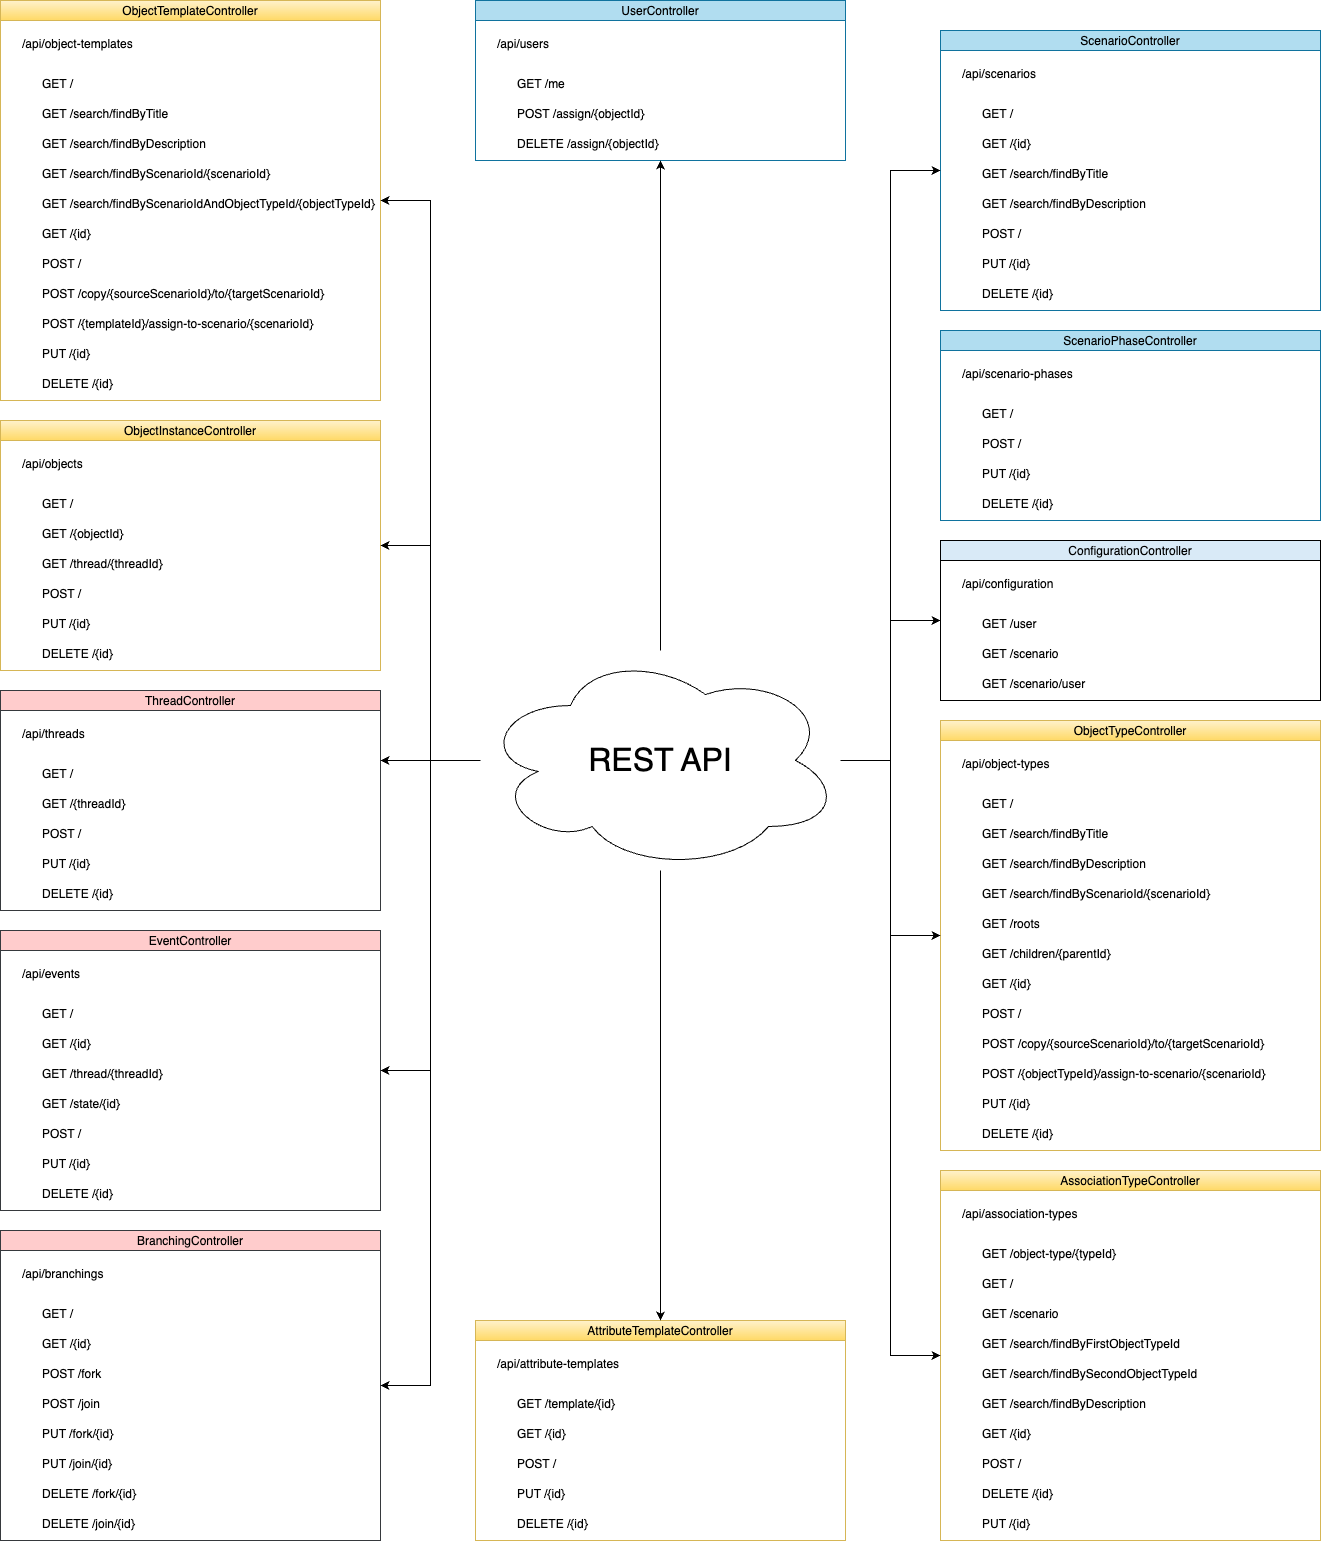
\includegraphics[width=0.99\textwidth]{resources/local/diagram-api.png}
    \caption{Diagram REST API}
\end{figure}

\section{Backend}

\subsection{Autoryzacja oraz uprawnienia}

Autoryzacja w naszej aplikacji obejmuje wszystkie endpointy, z wyjątkiem tych zdefiniowanych w liście odstępstw:
\begin{itemize}
    \item autoryzacja i zdarzenia z keycloacka
    \item dokumentacja
    \item monitorowanie stanu aplikacji
\end{itemize}
Odbywa się ona za pomocą tokenów JWT. Znajduje się on w kontekście bezpieczeństwa danego requesta, w obiekcie Authentication.
Dzięki danym znajdującym się w tokenie oraz wymaganym nagłówku posiadającym id scenariusza możemy sprawdzić czy użytkownik posiada uprawnienia edycji 
lub modyfikacji konkretnego scenariusza. Ważnym elementem architektury bezpieczeństwa naszej aplikacji jest CORS. 
Zablokuje on jakiekolwiek połączenia z niezdefiniowanych przez nas domen. Znacznie zwiększa to bezpieczeństwo aplikacji. 
w konfiguracja CORS-a definiujemy akceptowalne domeny, metody HTTP oraz nagłówki. W konfiguracji określamy także, że 
nie tworzymy oraz utrzymuje sesji HTTP dla użytkowników, ponieważ nie jest to potrzebne w sytuacji gdy wykorzystujemy mechanizm
tokenów. Za każdym razem posiadamy potrzebne dane autoryzacyjne. Wyłączamy także ochronę przed atakiem CSRF, która to jest domyślnie 
ustawiona w Spring Boot. Taki atak nie jest zagrożeniem w naszej polityce zarządzania sesjami.

Zdefiniowanie oddzielnych profili: deweloperskiego oraz produkcyjnego, pozwoliło nam na złagodzenie wielu warunków autoryzacyjnych
w sytuacji lokalnego uruchomienia aplikacji. 

\subsection{Obsługa błędów}

Błędy zwracane przez aplikację backendową wyglądają w następujący sposób:

\begin{lstlisting}[language=Java]
{
  "errorCode": "PHASE_OVERLAP",
  "errorGroup": "SCENARIO_PHASE",
  "values": ["12345"]
}
\end{lstlisting}

Wyjaśnienie poszczególnych części zwracanych błędów:
\begin{itemize}
    \item errorCode - klasa enum (wyliczeniowa), która zawiera w sobie szczegółowy kod błędu. Możemy ją potraktować jako
    ustandaryzowaną wiadomość wyjątku.
    \item errorGroup - klasa enum (wyliczeniowa), która mówi o tym z jaką częścią zapytania jest problem. Najczęściej odnosi się
    do konkretnej encji w bazie danych z nielicznymi wyjątkami.
    \item values - opcjonalna lista wartości kontekstowych, które można załączyć do błedu np. id obiektu w bazie. Ułatwia detekcje 
    problematycznego elementu.
\end{itemize}

W aplikacji posiadamy handlery, które odpowiadają za wychwytywanie błędów i transformowanie ich do jednolitej formy.
Możemy wyróżnić następujące typy handlerów:
\begin{itemize}
    \item bazodanowe: wychwytywanie błędów z bazy danych. Dopasowywujemy error code oraz error group na podstawie wiadomości wyjątku. Gdy dopasowanie nie
    jest możliwe zwracamy błąd serwera.
    \item walidacyjne: wychwytywanie błędów wynikających z błednych lub brakujących danych w requeście
    \item biznesowe: wychwytywanie błędów rzucanych w warstwie biznesowej.
\end{itemize}

\subsection{Repozytoria}

\subsection{Walidacja}

\subsection{Websocket}

\subsection{Paginacja}

\subsection{Testy}

\section{Frontend}

